% =====================================================================
%  OELLM — Observation of Earth + Language Model
%  Vertical A1 graduation-project poster (story-driven layout)
%  Compile:  pdflatex poster.tex   (twice)
% =====================================================================
\documentclass[final]{article}

\usepackage[a1paper, portrait, margin=12mm, top=10mm, bottom=10mm]{geometry}
\usepackage{fix-cm}
\usepackage[T1]{fontenc}
\usepackage[utf8]{inputenc}
\usepackage{lmodern}
\renewcommand{\familydefault}{\sfdefault}

\usepackage{graphicx}
\usepackage{xcolor}
\usepackage{colortbl}
\usepackage{tikz}
\usetikzlibrary{calc, positioning, backgrounds, shapes.geometric, shapes.arrows, fit, arrows.meta}
\usepackage{tabularx}
\usepackage{array}
\usepackage{booktabs}
\usepackage{ragged2e}
\usepackage{microtype}
\usepackage{caption}
\usepackage{etoolbox}
\usepackage[hidelinks]{hyperref}
\usepackage{calc}

% ---------- palette -----------------------------------------------------
\definecolor{oellmblue}{HTML}{0E3B6B}
\definecolor{oellmsky}{HTML}{1F77B4}
\definecolor{oellmorange}{HTML}{E07B19}
\definecolor{oellmgreen}{HTML}{2CA02C}
\definecolor{oellmred}{HTML}{C0392B}
\definecolor{oellmgold}{HTML}{D4A017}
\definecolor{paperbg}{HTML}{F7F4EE}
\definecolor{cardbg}{HTML}{FFFFFF}
\definecolor{cardline}{HTML}{B8B0A0}
\definecolor{soft}{HTML}{443F3A}
\definecolor{rowhi}{HTML}{FFF6E1}
\definecolor{rowok}{HTML}{DAF0DC}
\definecolor{barbg}{HTML}{EAE3D2}

\pagecolor{paperbg}

% ---------- typography sizes (A1 — readable from 1 m) --------------------
\newcommand{\fsTitle}{\fontsize{115}{122}\selectfont\bfseries}
\newcommand{\fsSubtitle}{\fontsize{42}{48}\selectfont}
\newcommand{\fsTagline}{\fontsize{30}{36}\selectfont}
\newcommand{\fsAuthors}{\fontsize{24}{30}\selectfont}
\newcommand{\fsBannerBig}{\fontsize{50}{56}\selectfont\bfseries}
\newcommand{\fsBanner}{\fontsize{24}{28}\selectfont}
\newcommand{\fsSection}{\fontsize{38}{44}\selectfont\bfseries}
\newcommand{\fsBlock}{\fontsize{24}{28}\selectfont\bfseries}
\newcommand{\fsLead}{\fontsize{20}{26}\selectfont}
\newcommand{\fsBody}{\fontsize{16}{20}\selectfont}
\newcommand{\fsSmall}{\fontsize{13}{16}\selectfont}
\newcommand{\fsTiny}{\fontsize{11}{13}\selectfont}

\setlength{\parindent}{0pt}
\setlength{\parskip}{2pt}

\captionsetup{font={small,sf}, labelfont={bf,color=oellmblue}, skip=1pt, justification=raggedright, singlelinecheck=false}

% ---------- card ---------------------------------------------------------
\setlength{\fboxsep}{5pt}
\setlength{\fboxrule}{0.6pt}
\newsavebox{\cardbox}
\newlength{\cardinner}
\newenvironment{card}{%
  \par\vspace{1pt}%
  \setlength{\cardinner}{\linewidth}%
  \addtolength{\cardinner}{-2\fboxsep}%
  \addtolength{\cardinner}{-2\fboxrule}%
  \noindent
  \begin{lrbox}{\cardbox}%
    \begin{minipage}{\cardinner}%
}{%
    \end{minipage}%
  \end{lrbox}%
  {\fcolorbox{cardline}{cardbg}{\usebox{\cardbox}}}%
  \par
}

\newcommand{\cardhead}[2]{%
  {\color{#1}\rule[2pt]{6pt}{20pt}}\;{\color{oellmblue}\fsBlock #2}\par
  \vspace{3pt}%
}

% Full-width section banner — slimmer
\newcommand{\sectionband}[3]{%
  \par\vspace{1pt}%
  \noindent\begin{tikzpicture}
    \fill[oellmblue] (0,0) rectangle (\linewidth, 1.70);
    \fill[#3] (0,0) rectangle (0.55, 1.70);
    \node[anchor=west, text=white] at (0.80, 0.85) {\fsSection #1\;\textcolor{#3}{$\bullet$}\;#2};
  \end{tikzpicture}\par\vspace{1pt}%
}

\newcommand{\statpill}[2]{%
  \begin{tikzpicture}[baseline=-2pt]
    \node[draw=oellmblue, line width=1.4pt, rounded corners=4pt,
          fill=white, inner xsep=14pt, inner ysep=8pt] {%
      {\bfseries\color{oellmblue}\fsBannerBig #1}\;{\color{soft}\fsBanner #2}%
    };
  \end{tikzpicture}%
}

\newcommand{\finding}[2]{%
  \par\smallskip
  \noindent\begin{tabular}{@{}p{7mm}@{\hspace{3mm}}p{\linewidth-12mm}@{}}
    \raisebox{2pt}{\color{#1}\rule{10pt}{10pt}} & \fsBody #2 \\
  \end{tabular}\par
}

\newcommand{\good}[1]{\textcolor{oellmgreen}{\textbf{#1}}}
\newcommand{\bad}[1]{\textcolor{oellmred}{\textbf{#1}}}
\newcommand{\hl}[1]{\cellcolor{rowhi}#1}
\renewcommand{\arraystretch}{1.15}

\pagestyle{empty}

\begin{document}
\sffamily
\fsBody

% =====================================================================
% HEADER  — slim band, large title, tight margins
% =====================================================================
\begin{tikzpicture}[remember picture, overlay]
  \fill[oellmblue] (current page.north west) rectangle ([yshift=-90mm]current page.north east);
  \fill[oellmorange] ([yshift=-88mm]current page.north west) rectangle ([yshift=-90mm]current page.north east);
  \begin{scope}
    \clip (current page.north west) rectangle ([yshift=-90mm]current page.north east);
    \foreach \i in {1,...,22}{
      \pgfmathsetmacro{\rx}{12 + \i*26}
      \pgfmathsetmacro{\ry}{8 + mod(\i*17,60)}
      \fill[oellmorange, opacity=0.20] ([xshift=\rx mm, yshift=-\ry mm]current page.north west) circle (1.4mm);
    }
  \end{scope}
  % QR code top-left, on a small white panel
  \node[anchor=north west, inner sep=0pt] at ([xshift=18mm, yshift=-16mm]current page.north west)
    {\fcolorbox{white}{white}{
\includegraphics[width=46mm]{qr.png}}};
  \node[anchor=north west, text=white, font=\fsSmall\bfseries] at ([xshift=18mm, yshift=-69mm]current page.north west)
    {Scan: dataset, code,};
  \node[anchor=north west, text=white, font=\fsSmall\bfseries] at ([xshift=18mm, yshift=-74mm]current page.north west)
    {\& reproducibility info};
\end{tikzpicture}

\vspace*{1mm}
\noindent\begin{minipage}{\linewidth}
  \color{white}\centering
  {\fsTitle OELLM}\\[-3mm]
  {\color{oellmorange}\rule{260mm}{1.8pt}}\\[2mm]
  {\fsSubtitle\bfseries Observation of Earth $\,\cdot\,$ Language Model}\\[3mm]
  {\fsTagline Dataset, Model \& Benchmark for Urban Understanding \& Cross-View Geolocalisation}\\[4mm]
  {\fsAuthors Ezel Bayraktar\,\textcolor{oellmorange}{$\bullet$}\,Alperen Demirci\,\textcolor{oellmorange}{$\bullet$}\,Mukhamediyar Amanzhol\,\textcolor{oellmorange}{$\bullet$}\,Adam Sattout}\\[1mm]
  {\fsSmall\color{paperbg!85!white} Graduation Project $\,\cdot\,$ 2026 $\,\cdot\,$ Qwen3.5-4B-VL}
\end{minipage}
\vspace{5mm}

\vspace{3mm}

% =====================================================================
% SECTION 1 — DATASET STORY
% =====================================================================
\sectionband{1}{The Dataset}{oellmorange}

\vspace{1mm}

% ---- Row 1a: Pipeline — hand-built TikZ, full-width
\begin{card}
\cardhead{oellmorange}{Pipeline~--- OSM seeds $\to$ paired imagery $\to$ deterministic MCQs}
\noindent
% Pipeline: full-card-width TikZ with 6 stages spanning \linewidth.
% Arrow gap = 10mm; box width = (W - 5*gap)/6.
\newlength{\pipeW}\setlength{\pipeW}{\linewidth}%
\addtolength{\pipeW}{-2\fboxsep}\addtolength{\pipeW}{-2\fboxrule}%
\newlength{\pipeBox}\setlength{\pipeBox}{\pipeW}%
\addtolength{\pipeBox}{-50mm}% 5 gaps of 10mm
\setlength{\pipeBox}{0.16667\pipeBox}% divide by 6
\newlength{\pipeStride}\setlength{\pipeStride}{\pipeBox}%
\addtolength{\pipeStride}{10mm}%
\begin{tikzpicture}[
    every node/.style={inner sep=0pt},
    stage/.style={
      draw=oellmblue, line width=0.9pt, rounded corners=4pt,
      fill=paperbg!55, minimum width=\pipeBox, minimum height=44mm,
      align=center, anchor=west
    },
    arr/.style={-{Latex[length=5mm, width=4.5mm]},
                line width=1.8pt, draw=oellmorange},
    badge/.style={
      circle, draw=oellmorange, fill=oellmorange, text=white,
      font=\fsSmall\bfseries, inner sep=2pt, minimum size=9mm
    }
  ]
  \foreach \i/\num/\ttl/\bdy in {%
    0/1/{Seed}/{40 cities\\32 countries\\6 continents},
    1/2/{OSM}/{Overpass tags:\\roads, land use,\\amenities, transit},
    2/3/{Imagery}/{1 satellite tile\\$+$ 4 Street-View\\headings},
    3/4/{MCQ gen}/{Deterministic\\templates over\\OSM facts},
    4/5/{Splits}/{\textsf{per\_city}\\\textsf{seen\_unseen}\\benchmark},
    5/6/{Dataset}/{4{,}168 locations\\14 task types\\5{,}240 bench}%
  }{
    \node[stage] (s\i) at (\i\pipeStride, 0) {};
    \node[anchor=north, font=\fsBlock, text=oellmblue]
      at ([yshift=-5mm]s\i.north) {\ttl};
    \node[anchor=center, font=\fsBody, text=soft, align=center]
      at ([yshift=-5mm]s\i.center) {\bdy};
    \node[badge] at ([xshift=5mm, yshift=-5mm]s\i.north west) {\num};
  }
  \foreach \i [evaluate=\i as \j using int(\i+1)] in {0,1,2,3,4}{
    \draw[arr] (s\i.east) -- (s\j.west);
  }
\end{tikzpicture}
\par\vspace{2pt}\fsSmall\color{soft}\raggedright
Each location pairs one $512{\times}512$ satellite tile with four Street-View
headings; every answer comes \textbf{deterministically from OpenStreetMap}~---
no annotators, bit-exact regenerable.
\end{card}

\vspace{1mm}

% ---- Row 1b: Geographic coverage map — 40 cities numbered, side index
\begin{card}
\cardhead{oellmorange}{Geographic coverage~--- 40 cities, 6 continents, 32 countries}
\centering
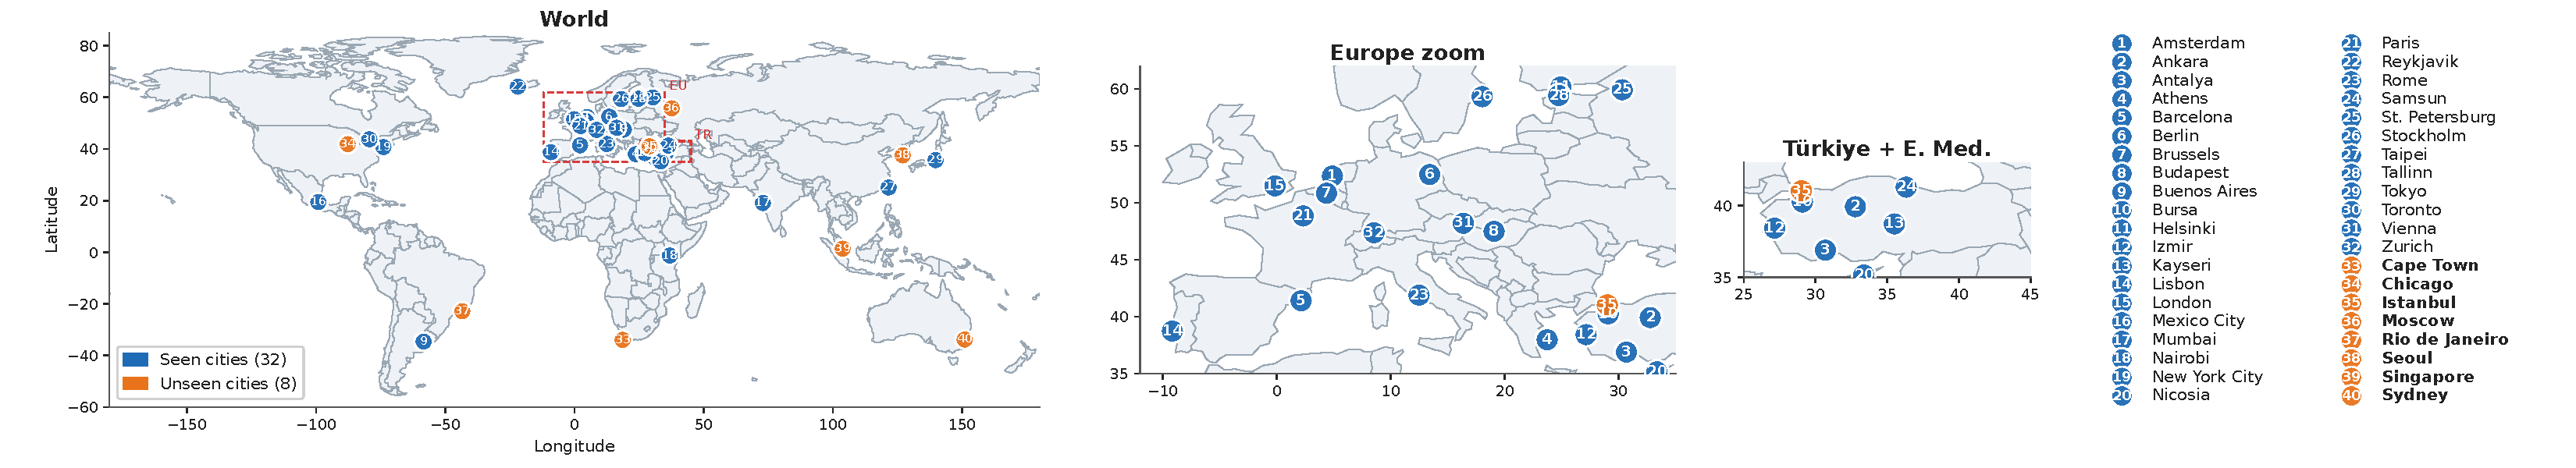
\includegraphics[width=\linewidth]{dataset_figures/fig11_geographic_scatter_poster.pdf}
\end{card}

\vspace{1mm}

% ---- Row 1d: Three example QAs — image (cropped to visual) + LaTeX-rendered Q&A beneath
% Trim values are (left, bottom, right, top) in native px before being converted to bp.
% land_use & urban_density: 1200x742, visual = top ~520px → trim bottom = 222px
% junction_type & mismatch_mcq_easy: 1200x772, visual = top ~540px → trim bottom = 232px
% mismatch_mcq_hard:        1200x1281, visual = top ~1080px → trim bottom = 200px
\newcommand{\qoption}[1]{\par\hangindent=14pt\hangafter=1 #1}
\newcommand{\qcorrect}[1]{\par\hangindent=14pt\hangafter=1\textbf{\color{oellmgreen}#1}}
\noindent
\begin{minipage}[t]{0.328\linewidth}
\begin{card}
\centering

\includegraphics[height=72mm, trim=0 235 0 0, clip, keepaspectratio]{examples/ex_mismatch_binary_hard.png}
\par\vspace{4pt}
\raggedright\fsSmall
\textbf{\color{oellmred}\textsf{camera\_direction}} \,$\cdot\,$ Izmir, Turkey\par\vspace{2pt}
\fsBody\textbf{Select the satellite image whose red arrow matches the viewing direction of this street view.}
\par\vspace{2pt}\fsBody
A.\,Image A \,$\cdot\,$\, \textbf{\color{oellmgreen}B.\,Image B\,[\,correct]} \,$\cdot\,$\, C.\,Image C \,$\cdot\,$\, D.\,Image D
\end{card}
\end{minipage}\hfill
\begin{minipage}[t]{0.328\linewidth}
\begin{card}
\centering

\includegraphics[height=72mm, trim=0 232 0 0, clip, keepaspectratio]{examples/ex_junction_type.png}
\par\vspace{4pt}
\raggedright\fsSmall
\textbf{\color{oellmsky}\textsf{junction\_type}} \,$\cdot\,$ Helsinki, Finland\par\vspace{2pt}
\fsBody\textbf{Looking at this location, how would you classify the road junction type?}
\par\vspace{2pt}\fsBody
A.\,Signalized intersection \,$\cdot\,$\, B.\,Roundabout \,$\cdot\,$\, \textbf{\color{oellmgreen}C.\,Unsignalized intersection\,[\,correct]} \,$\cdot\,$\, D.\,Grade-separated (overpass/underpass)
\end{card}
\end{minipage}\hfill
\begin{minipage}[t]{0.328\linewidth}
\begin{card}
\centering

\includegraphics[height=72mm, trim=0 232 0 0, clip, keepaspectratio]{examples/ex_mismatch_mcq_easy.png}
\par\vspace{4pt}
\raggedright\fsSmall
\textbf{\color{oellmred}\textsf{mismatch\_mcq\_easy}} \,$\cdot\,$ Sydney, Australia\par\vspace{2pt}
\fsBody\textbf{Which quadrant of the street view grid matches the marked satellite location?}
\par\vspace{2pt}\fsBody
\textbf{\color{oellmgreen}A.\,Top-Right\,[\,correct]} \,$\cdot\,$\, B.\,Bottom-Right \,$\cdot\,$\, C.\,Top-Left \,$\cdot\,$\, D.\,Bottom-Left
\end{card}
\end{minipage}


% =====================================================================
% SECTION 2 — METHOD & COMPOSITION
% =====================================================================
\sectionband{2}{Method \& Dataset Composition}{oellmgold}

% ---- Row 2: Training setup + Three splits — side by side
\noindent
\begin{minipage}[t]{0.495\linewidth}
\begin{card}
\cardhead{oellmsky}{Training setup}
\fsBody\renewcommand{\arraystretch}{1.25}
\begin{tabularx}{\linewidth}{@{}lX@{}}
\textbf{Model}    & Qwen3.5-4B-VL, vision SFT \\
\textbf{Adapter}  & LoRA $r{\in}\{16,32\}$, $\alpha{=}r$, all-linear \\
\textbf{Optim.}   & bs 86--96, lr $2.5{\times}10^{-4}$, cosine, 100 warmup \\
\textbf{Hardware} & RTX Pro 6000, 96\,GB, single GPU \\
\textbf{Eval}     & greedy, deterministic, \textsf{SEED}\,$=$\,3407 \\
\end{tabularx}
\par\vspace{3pt}\fsSmall\color{soft}\raggedright
PC-base 6\,ep; SU-base 8\,ep; ablations 5\,ep, early-stop patience 2.
Every run evaluated on the full 14-topic mix.
\end{card}
\end{minipage}\hfill
\begin{minipage}[t]{0.495\linewidth}
\begin{card}
\cardhead{oellmorange}{Three splits, one taxonomy}
\fsBody\renewcommand{\arraystretch}{1.25}\setlength{\tabcolsep}{4pt}
\begin{tabularx}{\linewidth}{@{}lrrX@{}}
\toprule
\textbf{Split} & \textbf{Train} & \textbf{Val} & \textbf{Generalisation question}\\
\midrule
{\color{oellmsky}\rule[0pt]{9pt}{9pt}}\;\textsf{per\_city}     & 26{,}931 & 6{,}984 & new loc., \emph{seen} cities \\
{\color{oellmorange}\rule[0pt]{9pt}{9pt}}\;\textsf{seen\_unseen} & 26{,}963 & 8{,}831 & 8 cities held out \\
{\color{oellmred}\rule[0pt]{9pt}{9pt}}\;\textsf{benchmark}     & 5{,}240\,pub & 5{,}240\,gold & disjoint from both \\
\bottomrule
\end{tabularx}
\par\vspace{3pt}\fsSmall\color{soft}\raggedright
\textbf{per\_city} = familiar contexts.
\textbf{seen\_unseen} = \emph{geographic generalisation}.
\textbf{benchmark} ships \texttt{answer:null} alongside a gold-labelled twin.
\end{card}
\end{minipage}


% =====================================================================
% SECTION 3 — RESULTS
% =====================================================================
\sectionband{3}{Results~--- training works, but transfer has limits}{oellmred}

% ---- Row 3a: Three columns — held-out benchmark | ABLATION MATRIX (hero) | ablation table
\noindent
\begin{minipage}[t]{0.27\linewidth}
\begin{card}
\cardhead{oellmblue}{Held-out benchmark~--- vs.\ 6 open VLMs}
\fsBody\color{soft}5{,}240 records $\,\cdot\,$ greedy decoding\par
\vspace{4pt}
\centering
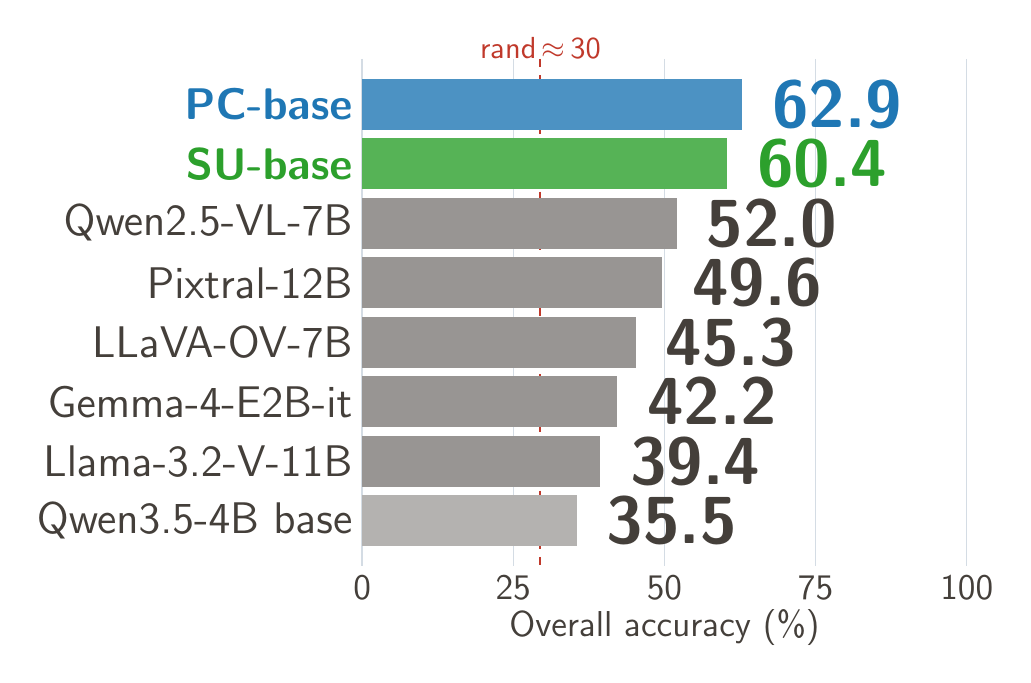
\begin{tikzpicture}[every node/.style={font=\fsBody}, x=1.2cm, y=0.72cm]
  \def\W{6.4}
  \foreach \v in {0,25,50,75,100}{
    \draw[oellmblue!18, line width=0.5pt] ({\W*\v/100},0.3) -- ({\W*\v/100},-8.65);
    \node[font=\fsSmall, text=soft, below] at ({\W*\v/100},-8.65) {\v};
  }
  \node[font=\fsSmall, text=soft, below] at (\W*0.5,-9.25) {Overall accuracy (\%)};
  \draw[oellmred, dashed, line width=0.7pt] ({\W*0.295},0.3) -- ({\W*0.295},-8.65);
  \node[font=\fsTiny, text=oellmred] at ({\W*0.295},0.5) {rand\,$\approx$\,30};

  % rows: name, value, color
  \node[anchor=east, font=\fsBody\bfseries, text=oellmsky] at (0,-0.50) {PC-base};
  \fill[oellmsky!80] (0,-0.95) rectangle ({\W*0.6286},-0.05);
  \node[anchor=west, font=\fsBlock, text=oellmsky] at ({\W*0.6286},-0.50) {\;\textbf{62.9}};

  \node[anchor=east, font=\fsBody\bfseries, text=oellmgreen] at (0,-1.55) {SU-base};
  \fill[oellmgreen!80] (0,-2.00) rectangle ({\W*0.6036},-1.10);
  \node[anchor=west, font=\fsBlock, text=oellmgreen] at ({\W*0.6036},-1.55) {\;\textbf{60.4}};

  \node[anchor=east, font=\fsBody, text=soft] at (0,-2.60) {Qwen2.5-VL-7B};
  \fill[soft!55] (0,-3.05) rectangle ({\W*0.5202},-2.15);
  \node[anchor=west, font=\fsBlock, text=soft] at ({\W*0.5202},-2.60) {\;52.0};

  \node[anchor=east, font=\fsBody, text=soft] at (0,-3.65) {Pixtral-12B};
  \fill[soft!55] (0,-4.10) rectangle ({\W*0.4964},-3.20);
  \node[anchor=west, font=\fsBlock, text=soft] at ({\W*0.4964},-3.65) {\;49.6};

  \node[anchor=east, font=\fsBody, text=soft] at (0,-4.70) {LLaVA-OV-7B};
  \fill[soft!55] (0,-5.15) rectangle ({\W*0.4525},-4.25);
  \node[anchor=west, font=\fsBlock, text=soft] at ({\W*0.4525},-4.70) {\;45.3};

  \node[anchor=east, font=\fsBody, text=soft] at (0,-5.75) {Gemma-4-E2B-it};
  \fill[soft!55] (0,-6.20) rectangle ({\W*0.4222},-5.30);
  \node[anchor=west, font=\fsBlock, text=soft] at ({\W*0.4222},-5.75) {\;42.2};

  \node[anchor=east, font=\fsBody, text=soft] at (0,-6.80) {Llama-3.2-V-11B};
  \fill[soft!55] (0,-7.25) rectangle ({\W*0.3939},-6.35);
  \node[anchor=west, font=\fsBlock, text=soft] at ({\W*0.3939},-6.80) {\;39.4};

  \node[anchor=east, font=\fsBody, text=soft] at (0,-7.85) {Qwen3.5-4B base};
  \fill[soft!40] (0,-8.30) rectangle ({\W*0.3548},-7.40);
  \node[anchor=west, font=\fsBlock, text=soft] at ({\W*0.3548},-7.85) {\;35.5};
\end{tikzpicture}
\par\vspace{4pt}\fsSmall\color{soft}\raggedright
\textbf{PC-base} and \textbf{SU-base} (ours, 4B params) beat all 6 open
VLMs incl.\ Qwen2.5-VL-7B and Pixtral-12B. SU-base is the honest
cross-city number; PC-base is best overall but overfits seen cities.
\end{card}
\end{minipage}\hfill
\begin{minipage}[t]{0.31\linewidth}
\begin{card}
\noindent{\color{oellmgreen}\rule[1pt]{5pt}{12pt}}\;{\color{oellmblue}\fsBody\bfseries Per-task accuracy \& ablations}\par\vspace{1pt}
\fsSmall\renewcommand{\arraystretch}{1.0}\setlength{\tabcolsep}{3pt}
\centering
\begin{tabular}{@{}lrrrrrrr@{}}
\toprule
\textbf{Task} & \textbf{Llama} & \textbf{LLaVA} & \textbf{Pix} & \textbf{Qwen2.5} & \textbf{Qwen3.5} & {\color{oellmgreen}\textbf{SU}} & {\color{oellmsky}\textbf{PC}}\\
\fsTiny & \fsTiny 11B & \fsTiny 7B & \fsTiny 12B & \fsTiny 7B & \fsTiny 4B & \fsTiny \textbf{ours} & \fsTiny \textbf{ours}\\
\midrule
Amenity Rich.       & \bad{24.2} & 35.2 & 32.1 & 31.4 & 24.7 & \good{56.5} & 53.2 \\
Building Height     & 49.0 & 57.9 & 59.0 & 60.5 & \bad{24.7} & 60.5 & \good{66.3} \\
Camera Direction    & 25.4 & 24.9 & 20.7 & \good{27.8} & \bad{7.6} & 26.1 & 24.5 \\
Green Space         & 49.8 & 76.9 & 66.0 & 84.7 & \bad{40.9} & 62.6 & \good{100.0} \\
Junction Type       & 44.6 & 53.6 & 49.4 & 61.1 & \bad{40.1} & 70.4 & \good{75.8} \\
Land Use            & 41.1 & 57.5 & 46.3 & 53.7 & \bad{29.0} & \good{75.1} & 73.6 \\
Mism. Bin.\ Easy    & 53.4 & 54.4 & 82.7 & \good{85.5} & \bad{51.8} & 55.6 & 53.0 \\
Mism. Bin.\ Hard    & \bad{44.2} & 44.9 & \good{87.2} & 64.9 & 45.1 & 49.6 & 44.4 \\
Mism. MCQ Easy      & \bad{23.5} & 29.2 & 26.4 & 42.3 & 31.6 & 73.2 & \good{76.5} \\
Mism. MCQ Hard      & \bad{20.4} & 23.8 & 28.0 & 37.3 & 30.9 & 59.6 & \good{60.1} \\
Road Surface        & 86.5 & 84.5 & 86.1 & 92.4 & \bad{71.6} & 75.3 & \good{96.0} \\
Road Type           & \bad{45.8} & 59.1 & 58.7 & 54.2 & 45.8 & \good{73.6} & 70.8 \\
Transit Density     & 33.7 & 28.7 & 31.8 & 27.3 & \bad{23.5} & 44.7 & \good{47.7} \\
Urban Density       & \bad{34.7} & 39.0 & 44.4 & 40.1 & 37.3 & 69.8 & \good{71.3} \\
\midrule
\textbf{Overall}    & 39.4 & 45.3 & 49.6 & 52.0 & \bad{35.5} & 60.4 & \good{\textbf{62.9}} \\
\midrule
\multicolumn{8}{@{}l}{\fsTiny\color{soft}\textbf{Ablations} (per\_city: All / Trained / Withheld)}\\
\multicolumn{4}{@{}l}{\fsTiny geo only (S-1)}      & \fsTiny 66.3 & \fsTiny 91.4 & \fsTiny 47.1 &\\
\multicolumn{4}{@{}l}{\fsTiny urban+cam (S-3)}     & \fsTiny 63.2 & \fsTiny 76.0 & \fsTiny 50.4 &\\
\multicolumn{4}{@{}l}{\fsTiny no camera (S-5)}     & \fsTiny 76.5 & \fsTiny 80.1 & \fsTiny\bad{29.9} &\\
\rowcolor{rowok}\multicolumn{4}{@{}l}{\fsTiny no-hard mism.\ (S-6)}  & \fsTiny\good{76.4} & \fsTiny 79.6 & \fsTiny\good{82.2} &\\
\bottomrule
\end{tabular}
\end{card}
\end{minipage}\hfill
\begin{minipage}[t]{0.40\linewidth}
\begin{card}
\cardhead{oellmred}{Transfer ladder}
\centering\vspace{2pt}
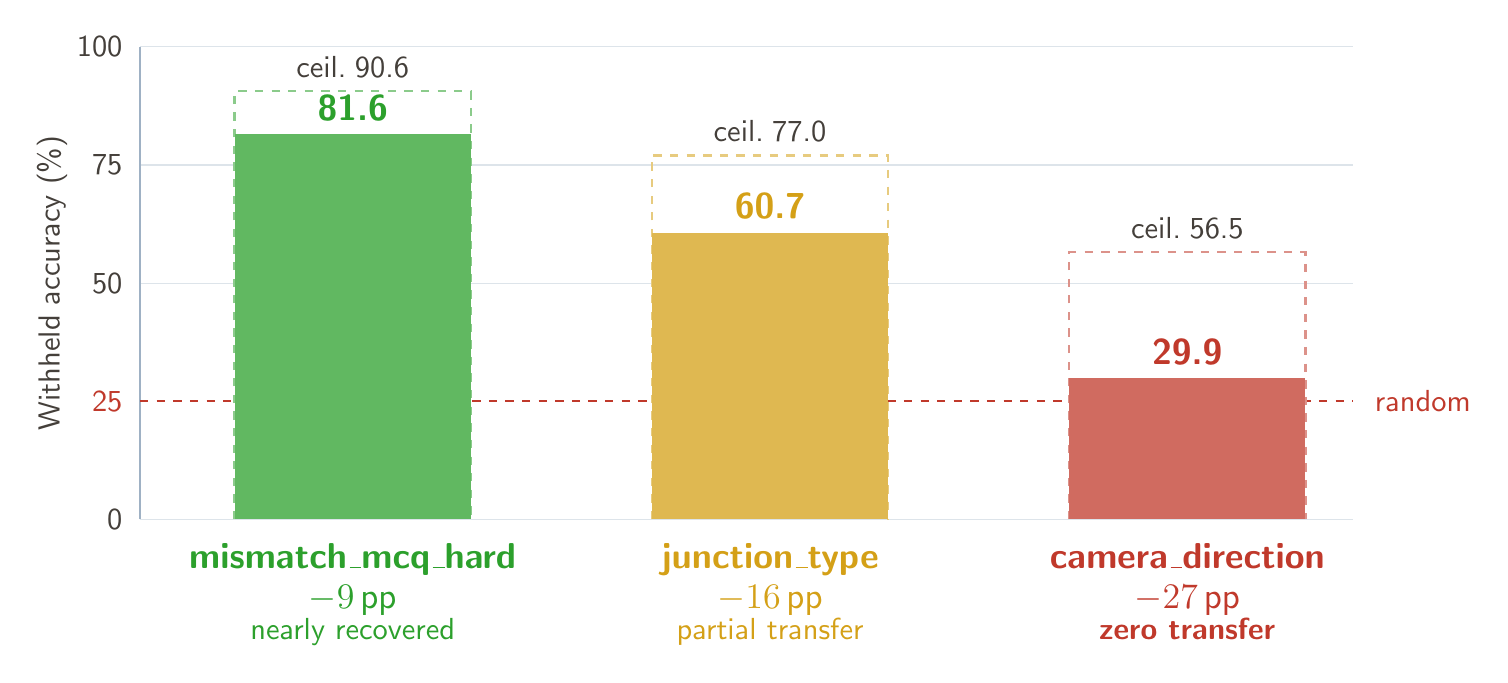
\begin{tikzpicture}[x=1cm, y=0.06cm]
  \def\AxX{0}\def\ColW{4.8}\def\Gap{0.5}\def\BarHW{1.5}\def\H{100}
  \pgfmathsetmacro{\xRight}{\AxX + 3*\ColW + 2*\Gap}
  \foreach \v in {0,50,75,100}{
    \draw[oellmblue!14, line width=0.4pt] (\AxX,\v) -- (\xRight,\v);
    \node[font=\fsTiny, text=soft, anchor=east] at (\AxX-0.10,\v) {\v};
  }
  \node[font=\fsTiny, text=oellmred, anchor=east] at (\AxX-0.10,25) {25};
  \draw[oellmblue!40, line width=0.5pt] (\AxX,0) -- (\AxX,\H);
  \node[font=\fsTiny, text=soft, rotate=90, anchor=south]
      at (\AxX-0.80,\H/2) {Withheld accuracy (\%)};
  \draw[oellmred, dashed, line width=0.6pt] (\AxX,25) -- (\xRight,25);
  \node[font=\fsTiny, text=oellmred, anchor=west]
      at (\xRight+0.05, 25) {\;random};
  \newcommand{\ladderCol}[7]{%
    \pgfmathsetmacro{\xC}{#1+\ColW/2}%
    \pgfmathsetmacro{\barL}{\xC-\BarHW}%
    \pgfmathsetmacro{\barR}{\xC+\BarHW}%
    \draw[#2!55, dashed, line width=0.8pt]
      (\barL,0) -- (\barL,#5) -- (\barR,#5) -- (\barR,0);
    \fill[#2!75] (\barL,0) rectangle (\barR,#4);
    \node[font=\fsSmall\bfseries, text=#2, anchor=south] at (\xC,#4+0.8) {#4};
    \node[font=\fsTiny, text=soft, anchor=south] at (\xC,#5+0.8) {ceil.\;#5};
    \node[font=\fsSmall\bfseries, text=#2, anchor=north, align=center]
      at (\xC,-3) {\textsf{#3}};
    \node[font=\fsSmall, text=#2, anchor=north] at (\xC,-12) {#6};
    \node[font=\fsTiny, text=#2, anchor=north, align=center]
      at (\xC,-19) {#7};
  }
  \ladderCol{\AxX+0.3}{oellmgreen}{mismatch\_mcq\_hard}{81.6}{90.6}{$-9$\,pp}{nearly recovered}
  \pgfmathsetmacro{\xMid}{\AxX+\ColW+\Gap+0.3}
  \ladderCol{\xMid}{oellmgold}{junction\_type}{60.7}{77.0}{$-16$\,pp}{partial transfer}
  \pgfmathsetmacro{\xLast}{\AxX+2*\ColW+2*\Gap+0.3}
  \ladderCol{\xLast}{oellmred}{camera\_direction}{29.9}{56.5}{$-27$\,pp}{\textbf{zero transfer}}
  \path (\xRight+0.85, 0);
\end{tikzpicture}
\par\vspace{1mm}\fsSmall\color{soft}\raggedright
3 withheld-task outcomes vs ceiling (PC-base on the same topic).
\textsf{mismatch\_mcq\_hard} nearly recovers via easy-variant transfer;
\textsf{junction\_type} partially transfers from geo supervision;
\textsf{camera\_direction} has no transfer source in this dataset.
\end{card}
\end{minipage}

\vspace{0.5mm}

% ---- Row 3d: Within-family transfer — full width
{\noindent
\begin{minipage}{\linewidth}
\begin{card}
\noindent{\color{oellmsky}\rule[1pt]{5pt}{12pt}}\;{\color{oellmblue}\fsBody\bfseries Within-family transfer~--- easy carries hard}\par\vspace{1pt}
\centering
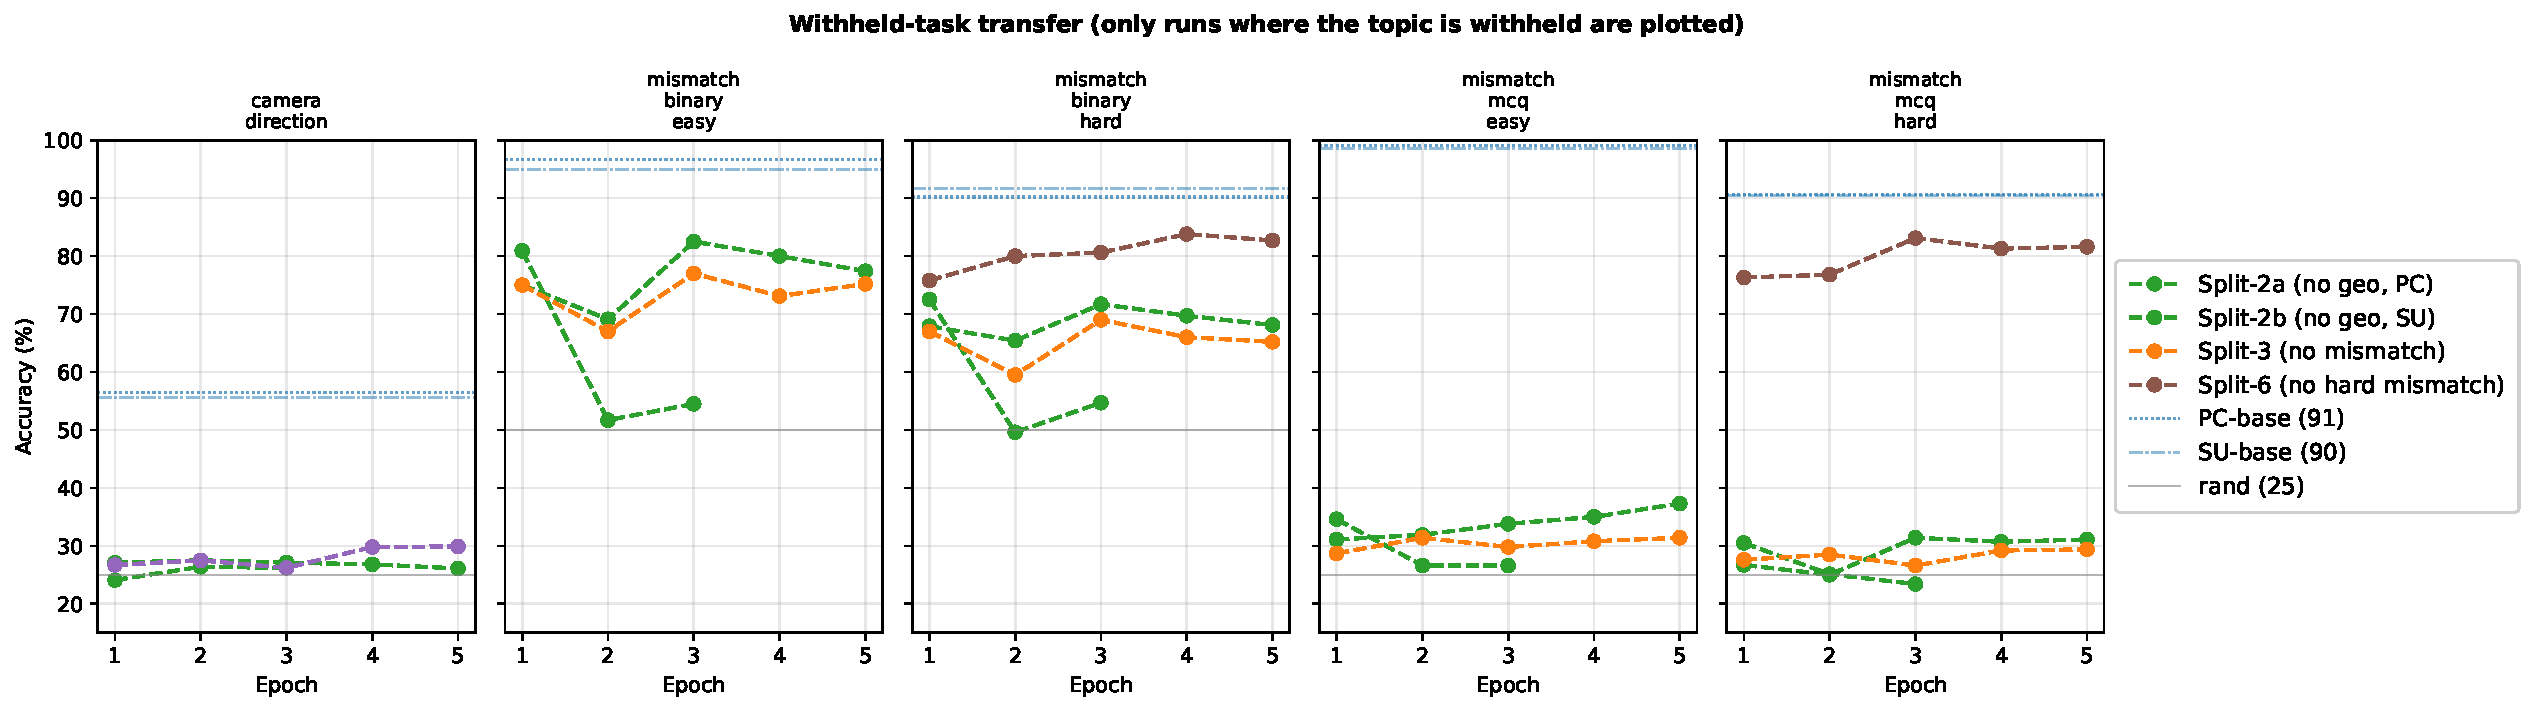
\includegraphics[width=\linewidth, height=130mm, keepaspectratio]{ablation_figures/fig3_geo_withheld.pdf}
\end{card}
\end{minipage}}

% =====================================================================
% FOOTER (compact)
% =====================================================================
\vspace*{0.5mm}
\begin{tikzpicture}[remember picture, overlay]
  \fill[oellmblue] ([yshift=9mm]current page.south west) rectangle (current page.south east);
  \fill[oellmorange] ([yshift=10mm]current page.south west) rectangle ([yshift=9mm]current page.south east);
  \node[anchor=center, text=white, font=\fsSmall] at ([yshift=4.5mm]current page.south)
    {\textbf{Dataset \& code}\;\textsf{github.com/\,\textellipsis\,/OELLM}\quad
     \textbf{Release}\;\textsf{EODATA\_compressed\_final}\,$\sim$7\,GB\quad
     \textbf{Contact}\;ezel964@icloud.com\quad
     {\color{paperbg!85!white}OELLM 2026 $\,\cdot\,$ Qwen3.5-4B-VL $\,\cdot\,$ RTX Pro 6000}};
\end{tikzpicture}

\end{document}
